\chapter{Telas da Aplicação}

\subsection{Tela Principal}

\begin{figure}[!h]
 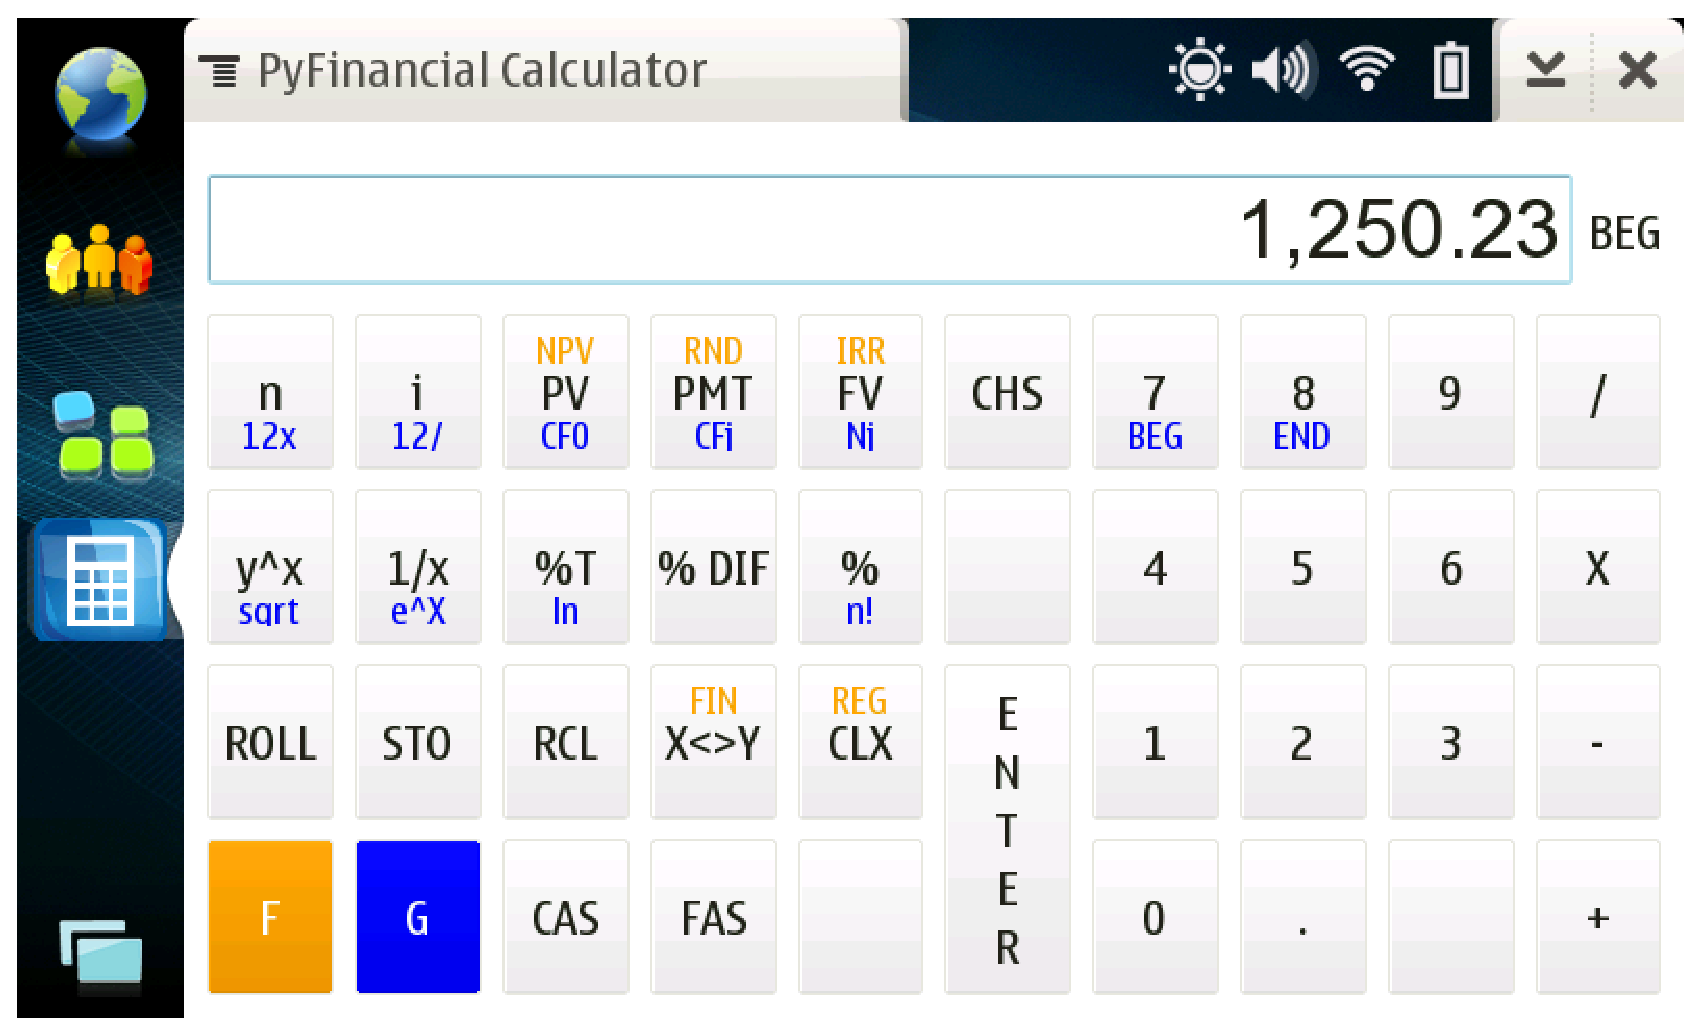
\includegraphics[scale=0.55]{tela_principal.eps}
 \caption{\it Tela principal da calculadora.} \label{tab:tela_principal}
\end{figure}

Tela principal da aplicação que permite o usuário ter acesso a todas as funcionalidade
implementadas pela calculadora. É atraves do mostrador da calculadora que o usuário irá
receber o resultado da maioria das funcões.


\subsection{Tela de Exceção}

\begin{figure}[!h]
 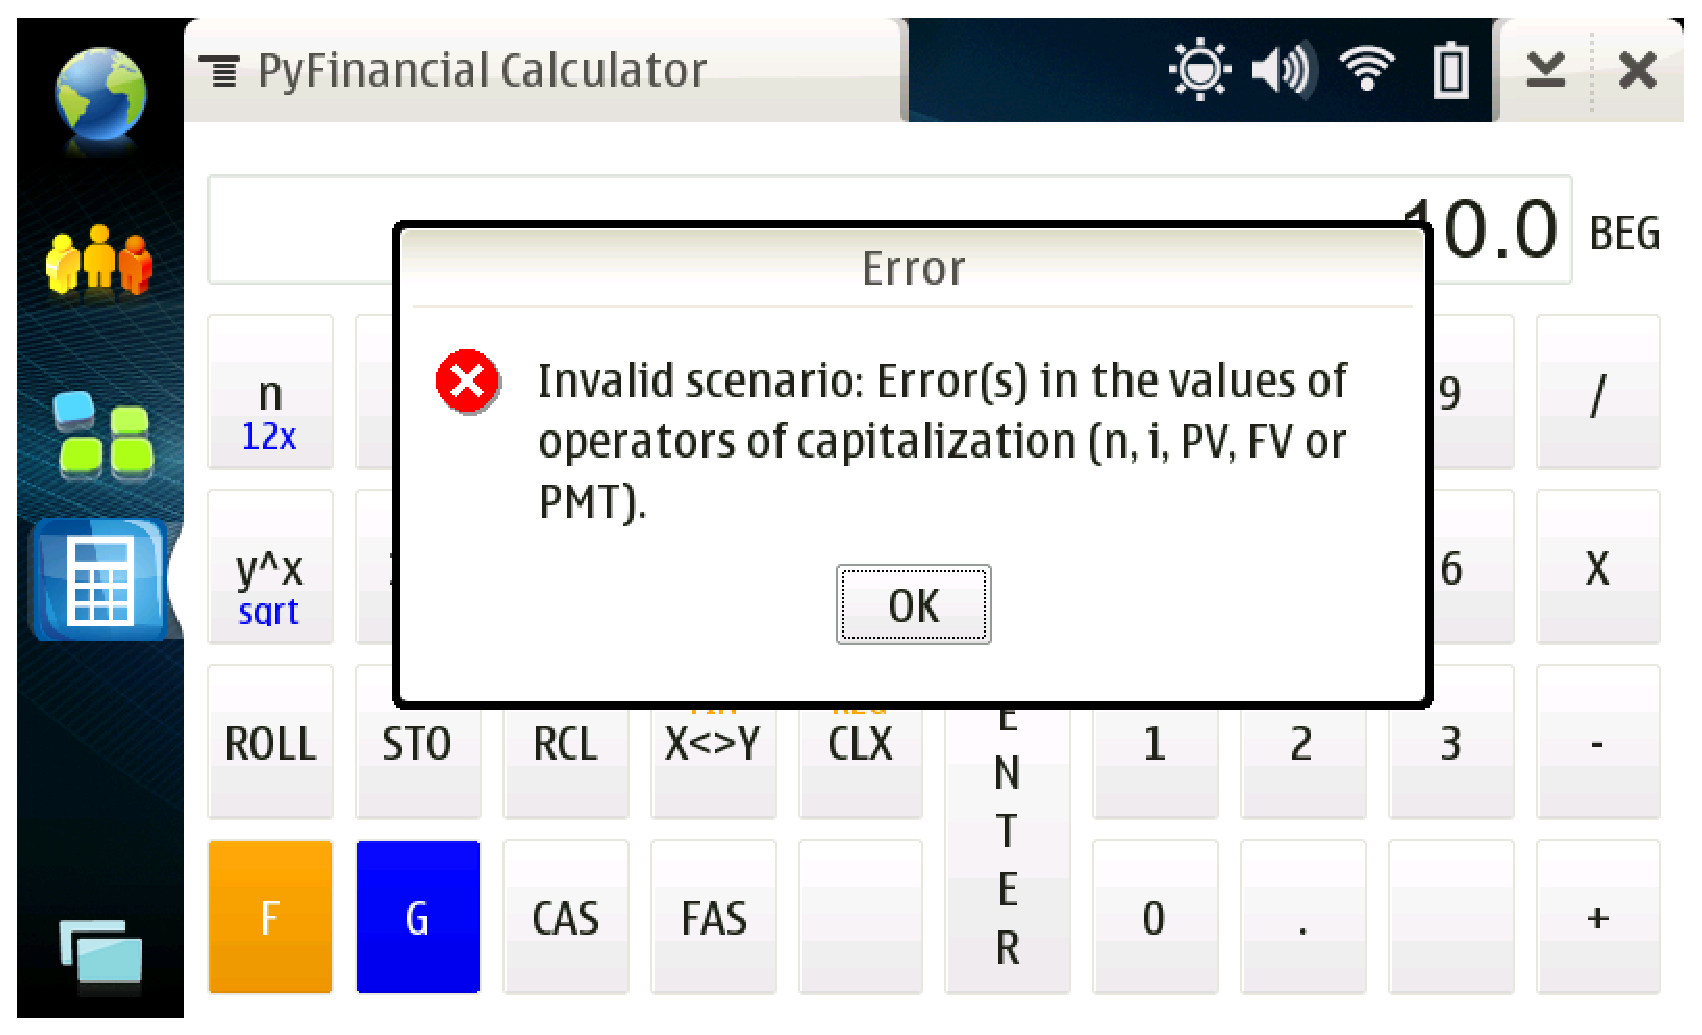
\includegraphics[scale=0.55]{tela_error.eps}
 \caption{\it Tela de exceção.} \label{tab:tela_error}
\end{figure}

Tela principal após uma exceção ser gerada. Um \textit{box} é aberto para mostrar ao usuário a
mensagem de erro.


\subsection{Telas de Amortização}

\begin{figure}[!h]
 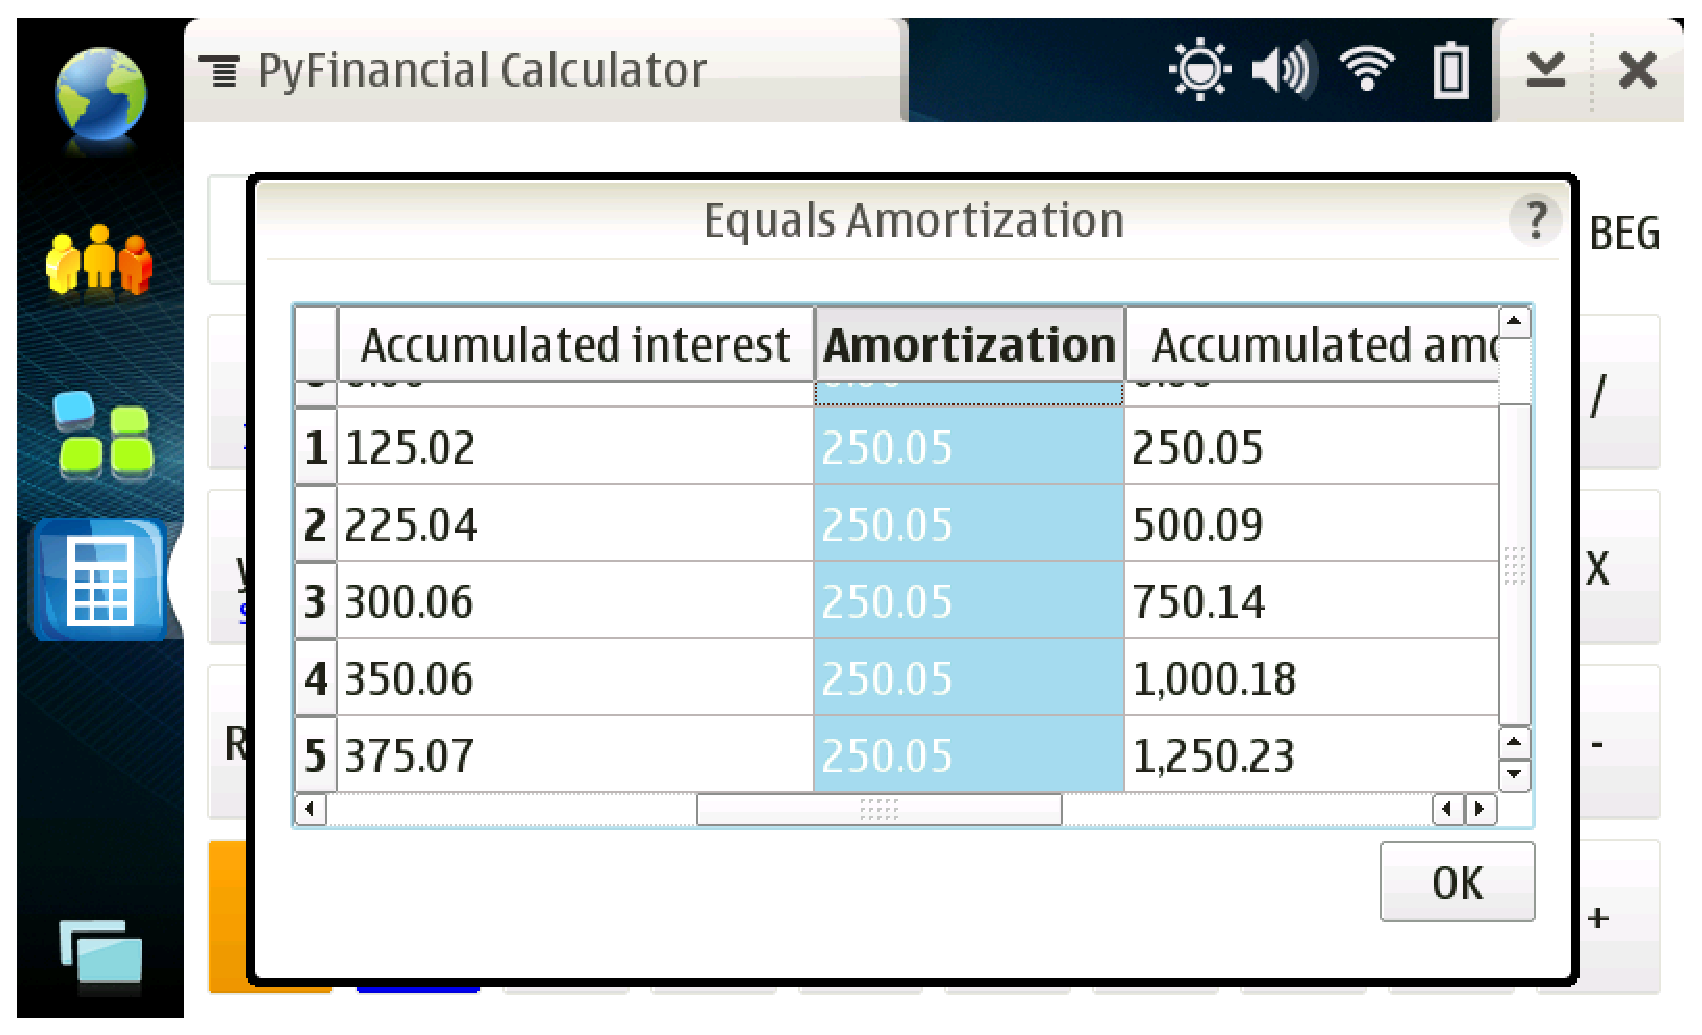
\includegraphics[scale=0.55]{tela_cas.eps}
 \caption{\it Tela de amortização constante.} \label{tab:tela_cas}
\end{figure}

\begin{figure}[!h]
 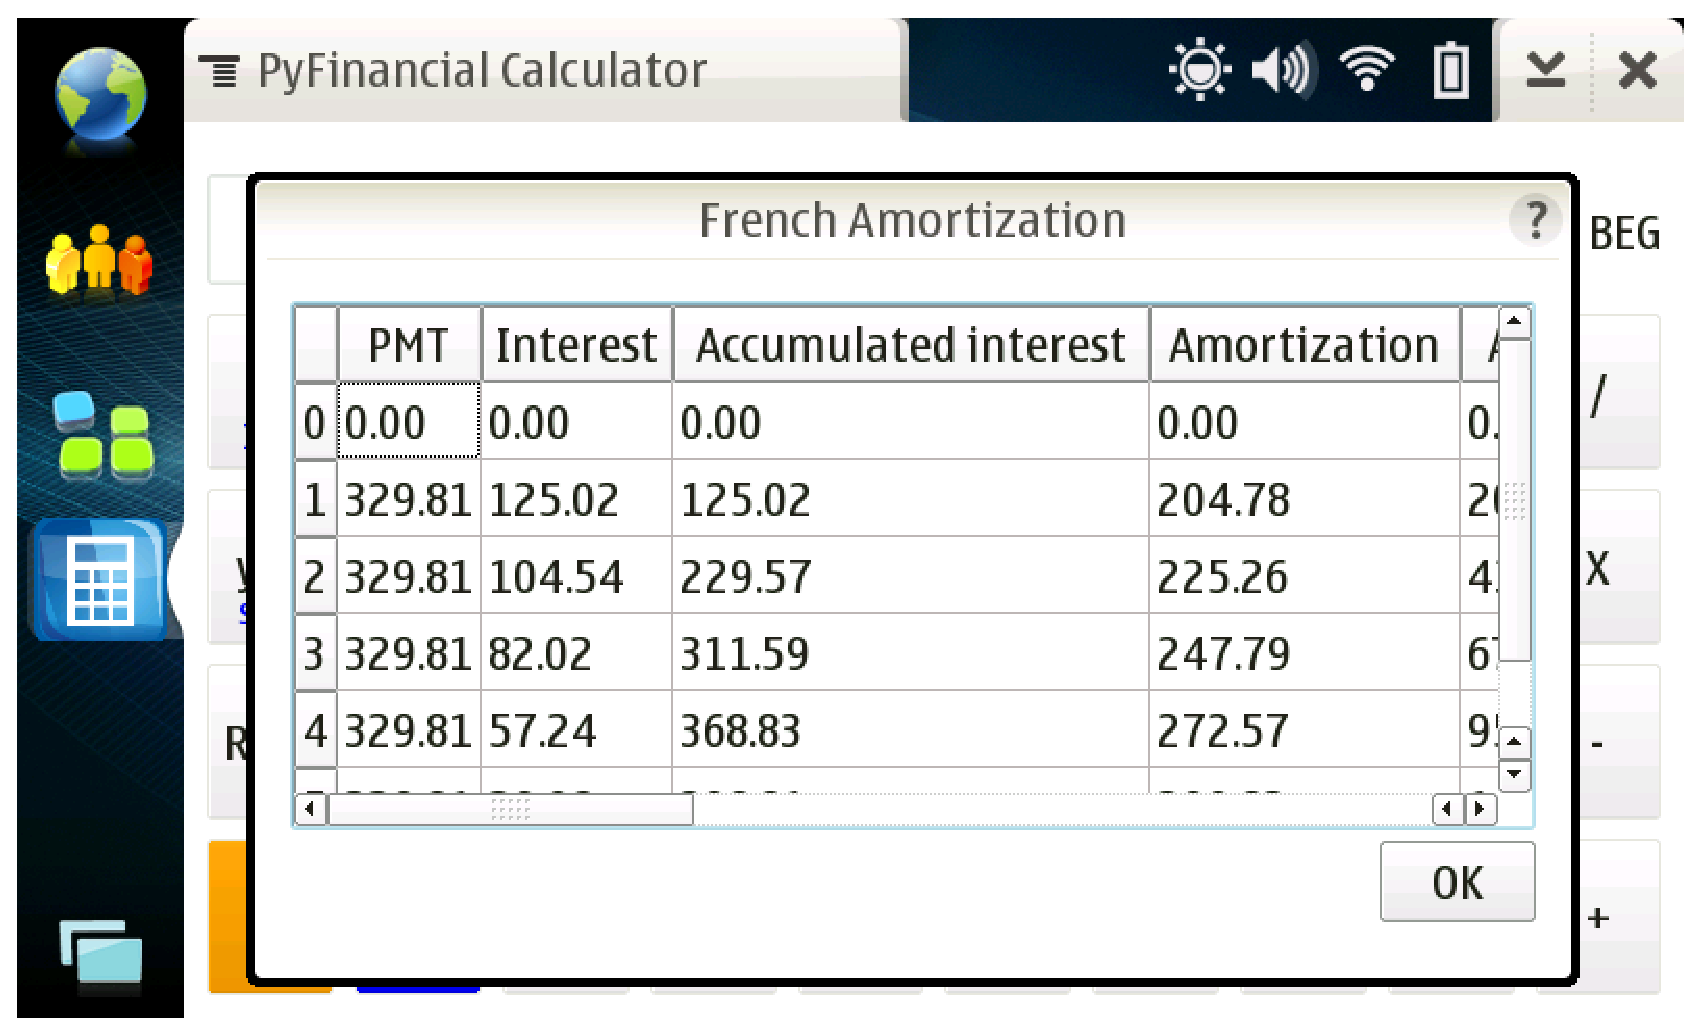
\includegraphics[scale=0.55]{tela_fas.eps}
 \caption{\it Tela de amortização francesa.} \label{tab:tela_fas}
\end{figure}


As telas de amortização apresentam no formato de tabela o resultado de uma calculo de
amortização constate ou francesa.


\subsection{Telas de Recall}

\begin{figure}[!h]
 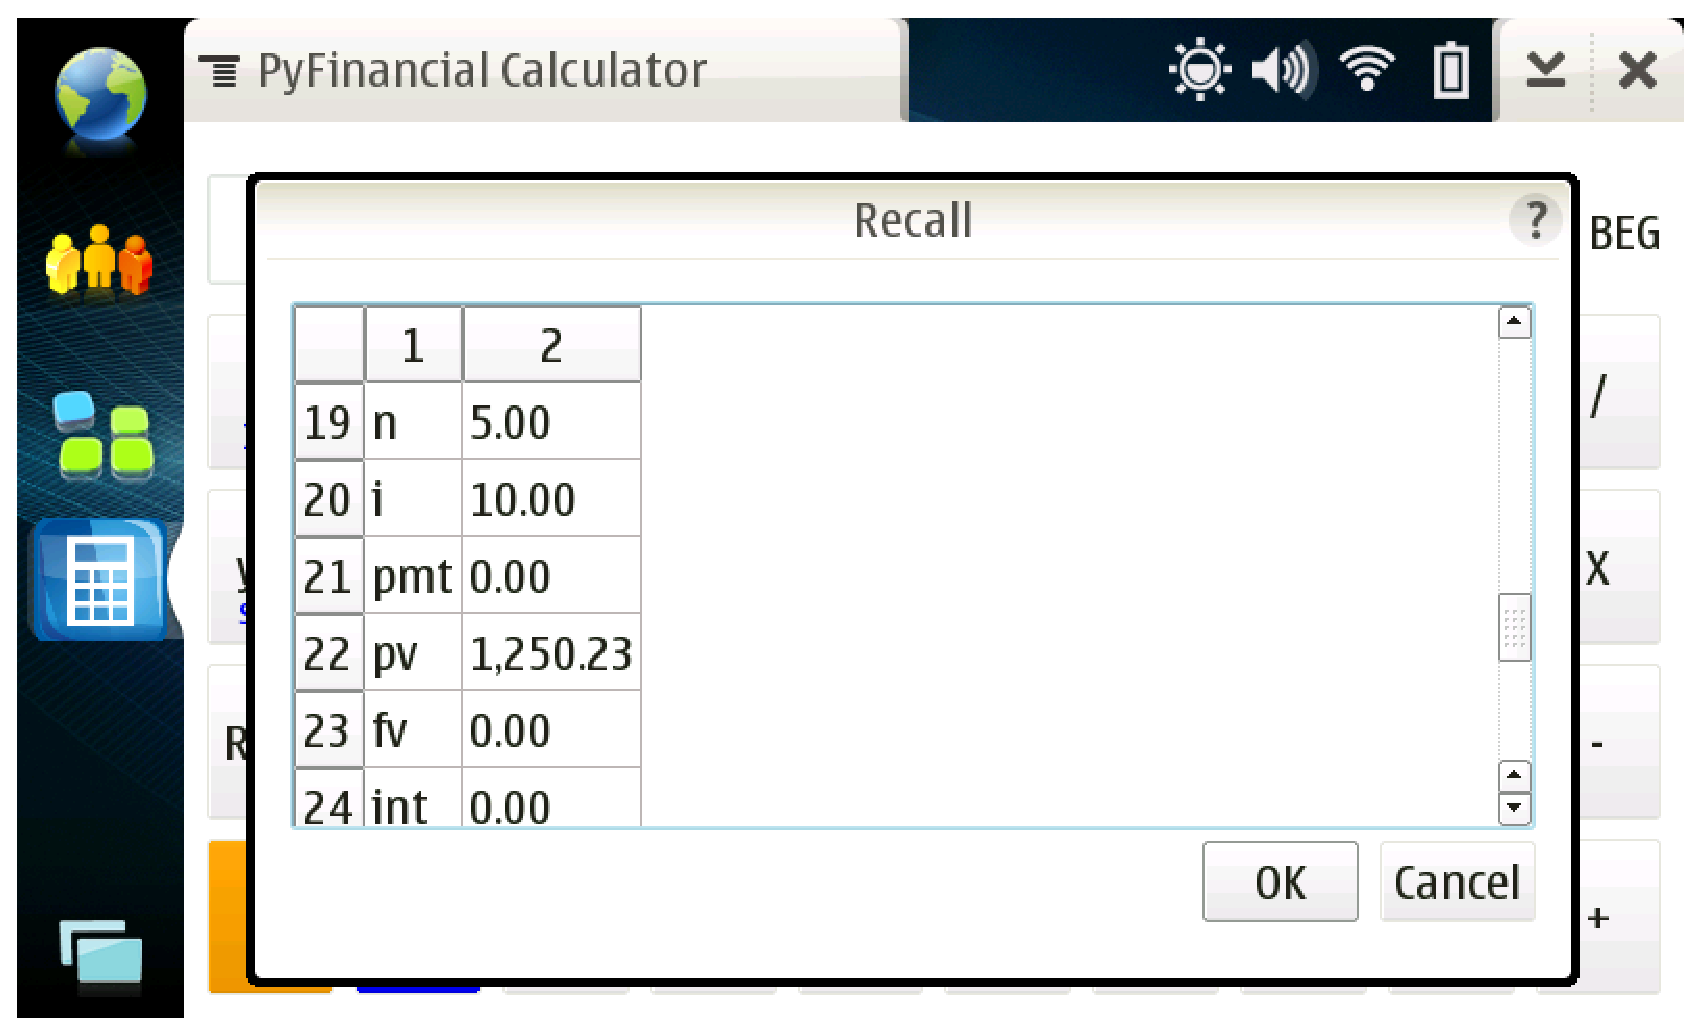
\includegraphics[scale=0.55]{tela_recall.eps}
 \caption{\it Tela de \textit{recall} de registradores.} \label{tab:tela_recall}
\end{figure}

A tela de \textit{Recall} serve para o usuário selecionar um registrador da calculadora e o valor
dele será mandado para o mostrador quando o ele clicar em \textit{OK}. Dessa forma, a pessoa poderá
utilizar o valor de um registrador em novos cálculos.

Existe também uma tela de \textit{Store}, com o mesmo design da tela de \textit{Recall}, que permite que o
usuário faça o inverso, ou seja, armazene o valor do mostrador em um registrador.